%++++++++++++++++++++++++++++++++++++++++
% Don't modify this section unless you know what you're doing!
\documentclass[letterpaper,12pt]{article}
\usepackage{tabularx} % extra features for tabular environment
\usepackage{amsmath}  % improve math presentation
\usepackage{amssymb}
\usepackage{graphicx} % takes care of graphic including machinery
\usepackage{pgfplots}
\pgfplotsset{width=10cm,compat=1.9}
\usepackage[margin=1in,letterpaper]{geometry} % decreases margins
\usepackage{cite} % takes care of citations
\usepackage[final]{hyperref} % adds hyper links inside the generated pdf file
\usepackage{tikz}
\usepackage{xcolor}
\usepackage{listings}
\usepackage{url}
\usepackage{tikz}
\usepackage{tzplot}
\renewcommand{\vec}[1]{\boldsymbol{#1}}
\hypersetup{
	colorlinks=true,       % false: boxed links; true: colored links
	linkcolor=blue,        % color of internal links
	citecolor=blue,        % color of links to bibliography
	filecolor=magenta,     % color of file links
	urlcolor=blue         
}
%++++++++++++++++++++++++++++++++++++++++

\title{PRML-Assignment 2}
\author{Rohith Ingilela,  EE19BTECH11005 }
\date{April 8, 2023}

\begin{document}

\maketitle

\section{Problem Statement}

In Figure \ref*{fig:fig1}, $ABCD$ is a parallelogram, $AE \perp DC$
and $CF \perp AD$. If $AB = 16 \hspace{0.1cm} cm$, $AE = 8 \hspace{0.1cm} cm$ and
$CF = 10 \hspace{0.1cm} cm$, find $AD$. Construct the paralellogram.

\begin{figure}[!ht]
\centering

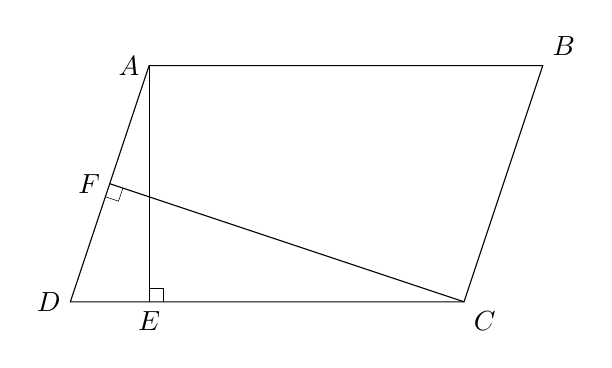
\begin{tikzpicture}
% triangle
\tzcoors(0,0)(D){$D$}[180](5,0)(C){$C$}[-45](6,3)(B){$B$}[45](1,3)(A){$A$}[180](1,0)(E){$E$}[-90](0.5,1.5)(F){$F$}[180];
\tzpolygon(A){}(B){}(C){}(D){};
\tzpolygon(A){}(E){};
\tzpolygon(C){}(F){};
% angle marks
\tzrightanglemark(D)(F)(C){}
\tzrightanglemark(A)(E)(C){}
\end{tikzpicture}

\caption{Parallelogram ABCD}
\label{fig:fig1}
\end{figure}
\section{Solution}

Given,
\begin{equation}
    AE \perp DC \implies (\Vec{A} - \Vec{E})^T (\Vec{C} - \Vec{D}) = 0
\end{equation}
\begin{equation}
    CF \perp AD \implies (\Vec{C} - \Vec{F})^T (\Vec{A} - \Vec{D}) = 0
\end{equation}
\begin{equation}
    \|AB\| = \|\Vec{A} - \Vec{B}\| = 16 cm
\end{equation}
\begin{equation}
    \|AE\| = \|\Vec{A} - \Vec{E}\| = 8 cm
\end{equation}
\begin{equation}
    \|CF\| = \|\Vec{C} - \Vec{F}\| = 10 cm
\end{equation}
To find: $\|AD\|$

\clearpage
We know that,
\begin{center}
    $Ar(ABCD) = \|AD\|\times\|CF\| = \|AE\|\times\|CD\|$ \\
\end{center}
\begin{center}
    $\|AD\| \times 10 = 8 \times 16 = 128$
\end{center}
\begin{equation}
    \|AD\| = 12.8 \text{ } cm
\end{equation}
\begin{center}
    $\|AD\| = \|\Vec{A} - \Vec{D}\| = 12.8 \text{ } cm$
\end{center}

To find: $\Vec{A}$ \\ \\
Let $\Vec{A} = \begin{pmatrix} x \\ 8 \end{pmatrix}$

\begin{center}
    $\|\Vec{A}\| = 12.8$
\end{center}
\begin{center}
    $x^2 + 8^2 = 12.8^2$
\end{center}
\begin{equation}
    x \approx 10
\end{equation}
\begin{equation}
    \Vec{A} = \begin{pmatrix} 10 \\ 8 \end{pmatrix}
\end{equation}
To find: $\Vec{F}$ \\ \\
Given,
\begin{center}
    $\|CF\| = \|\Vec{F} - \Vec{C}\| = 10$
\end{center}
Squaring on both sides,
\begin{center}
    $\Vec{F}^T\Vec{F} - 2\Vec{C}^T\Vec{F} + \Vec{C}^T\Vec{C} = 100$
\end{center}
\begin{equation}
    2\Vec{C}^T\Vec{F} - \Vec{F}^T\Vec{F} = 156 \hspace{0.6cm} (\because \Vec{C}^T\Vec{C} = 256)
\label{eqn1}
\end{equation}

From Figure \ref{fig:fig1}, $DF \perp CF$
\begin{center}
    $(\Vec{F}-\Vec{D})^T(\Vec{C}-\Vec{F}) = 0$
\end{center}
\begin{equation}
    \Vec{C}^T\Vec{F} - \Vec{F}^T\Vec{F} = 0
\label{eqn2}
\end{equation}
From (\ref*{eqn1}) and (\ref*{eqn2}),
\begin{equation}
    \Vec{C}^T\Vec{F} = 156
\label{eqn3}
\end{equation}

\clearpage

Equation of line passing through AD:
\begin{center}
    Direction vector, $\Vec{m} = \begin{pmatrix} 10 \\ 8 \end{pmatrix}$
\end{center}
Normal vector,
\begin{center}
    $\implies \Vec{n} = \begin{pmatrix} -8 \\ 10 \end{pmatrix}$
\end{center}
Equation of line passing through D with normal vector n is
\begin{center}
    $\Vec{n}^T(\Vec{x} - \Vec{D}) = 0$
\end{center}
Since $\Vec{F}$ passes through AD,
\begin{equation}
    \Vec{n}^T\Vec{F} = 0
\label{eqn4}
\end{equation}

From (\ref*{eqn3}) and (\ref*{eqn4}),
\begin{center}
    $\begin{pmatrix}\Vec{C}^T \\ \Vec{n}^T \end{pmatrix}\Vec{F} = \begin{pmatrix} 156 \\ 0 \end{pmatrix}$
\end{center}
Substituting values of $\Vec{C}$ and $\Vec{n}$
\begin{center}
    $\begin{pmatrix}16 & 0 \\ -8 & 10 \end{pmatrix}\Vec{F} = \begin{pmatrix} 156 \\ 0 \end{pmatrix}$
\end{center}
\begin{center}
    $\Vec{F} = \begin{pmatrix}16 & 0 \\ -8 & 10 \end{pmatrix}^{-1}\begin{pmatrix} 156 \\ 0 \end{pmatrix}$
\end{center}
\begin{center}
    $\Vec{F} = \frac{1}{160}\begin{pmatrix}10 & 0 \\ 8 & 16 \end{pmatrix}\begin{pmatrix} 156 \\ 0 \end{pmatrix}$
\end{center}
\begin{equation}
    \Vec{F} = \begin{pmatrix}9.75 \\ 7.8\end{pmatrix}
\end{equation}

\clearpage

\section{Code}
\url{https://github.com/1R0H1TH/PRML/blob/main/9.9.2.1/codes/9.9.2.1.py}

\section{Plot}
The above code plots Figure \ref{fig:fig2}.
\begin{figure}[!ht]
\centering
\includegraphics[width=0.75\columnwidth]{figs/Figure_1.png}
\caption{Parallelogram ABCD}
\label{fig:fig2}
\end{figure}.


\end{document}
